%Sella
\begin{figure}[h]
	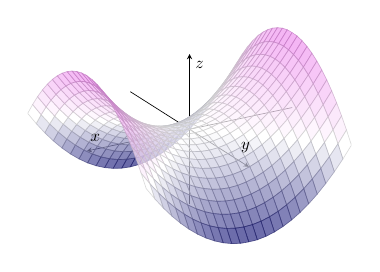
\begin{tikzpicture}[scale=0.6]
		\begin{axis}[view={150}{30}, axis lines=middle, xlabel=$x$, ylabel=$y$, zlabel=$z$,
			ticks=none,
			colormap/violet]
		\addplot3[surf,domain=-2:2,domain y=-2:2,opacity=0.7] 
		{x^2 - y^2}; % Funzione con un punto di sella in (0,0)
		\end{axis}
	\end{tikzpicture}
\end{figure}